\documentclass{pre-tfg}

\usepackage{listings}
\usepackage{formular}
\usepackage[pdftex]{graphicx}
\usepackage[toc,page]{appendix}

\showhelp  % comenta o borra para eliminar ayudas

\title{ClassifiAds: Sistema de clasificación de páginas web con respecto a Banners}
\author{Alberto Aranda García y Cristian Gómez Portes}
\advisorFirst{Luis Rodríguez Benitez}
\advisorDepartment{Departamento de Tecnologías y Sistemas de Información}
\advisorSecond{}
\intensification{COMPUTACIÓN}
\docdate{2017}{Enero}


\DeclareGraphicsExtensions{.pdf,.png,.jpg}

\usepackage{color}
\definecolor{gray97}{gray}{.97}
\definecolor{gray75}{gray}{.75}
\definecolor{gray45}{gray}{.45}
\definecolor{dkgreen}{rgb}{0,0.6,0}
\definecolor{gray}{rgb}{0.5,0.5,0.5}
\definecolor{mauve}{rgb}{0.58,0,0.82}
\definecolor{light-gray}{gray}{0.25}

\lstset{ frame=Ltb,
     framerule=0pt,
     aboveskip=0.5cm,
     framextopmargin=3pt,
     framexbottommargin=3pt,
     framexleftmargin=0.4cm,
     framesep=0pt,
     rulesep=.4pt,
     backgroundcolor=\color{gray97},
     rulesepcolor=\color{black},
     %
     stringstyle=\ttfamily,
     showstringspaces = false,
     basicstyle=\small\ttfamily,
     commentstyle=\color{gray45},
     keywordstyle=\bfseries,
     %
     numbers=left,
     numbersep=15pt,
     numberstyle=\tiny,
     numberfirstline = false,
     breaklines=true,
   }

% minimizar fragmentado de listados
\lstnewenvironment{listing}[1][]
   {\lstset{#1}\pagebreak[0]}{\pagebreak[0]}

\lstdefinestyle{consola}
   {basicstyle=\scriptsize\bf\ttfamily,
    backgroundcolor=\color{gray75},
   }

% lenguaje que se utilizará
\lstdefinestyle{java}{
  language=Java,
  aboveskip=3mm,
  belowskip=3mm,
  showstringspaces=false,
  columns=flexible,
  basicstyle={\footnotesize\ttfamily},
  numberstyle={\tiny},
  numbers=left,
  keywordstyle=\color{blue},
  commentstyle=\color{dkgreen},
  stringstyle=\color{mauve},
  breaklines=true,
  breakatwhitespace=true,
  tabsize=3
}

\renewcommand{\lstlistlistingname}{Índice de listado de código}

\begin{document}

\maketitle
\tableofcontents
\pagebreak
\listoffigures
\pagebreak
\lstlistoflistings

\newpage

\section{OBJETIVOS}

El presente proyecto trata de clasificar con un sistema multi-agente ciertas páginas con respecto al número de anuncios o ``banners'' y sus tipos (contenido publicitario, sexual, etc.) asociadas a éstas.

El sistema multiagente contará con cuatro agentes, los cuales recogerán información de diferentes páginas (los anuncios o ``banners'' que encuentre) para enviárselo a otro agente, que estará en una capa inferior. Éste se encargará de procesar esa información para establecer el ranking y comprobar de qué tipo son los anuncios. Una vez tengamos la información procesada, ésta será enviada a otro agente, en una capa más inferior, que será el encargado de mostrar el ranking a el usuario mediante una interfaz o similar.

Con respecto a la tecnología a utilizar, se usará Java como lenguaje de programación y Jade, un marco de software que simplifica la implementación de sistemas multi-agentes en Java -- en \cite{bellifemine2002jade} se puede encontrar más información sobre esta plataforma. Además, se utilizarán las siguientes librerías para facilitar el desarrollo del proyecto:

\begin{itemize}
 \item \textit{Jsoup}: librería utilizada para trabajar con HTML. Sitio de descarga: \url{https://jsoup.org/download}.
\item  \textit{Regex}: librería para trabajar con expresiones regulares. Viene incluida en el paquete ``util'' de Java.
\end{itemize}

\section{ESTRUCTURA DEL SMA}
El sistema multiagente desarrollado se compone de seis agentes como se especificó en el apartado anterior. Los cuatro agentes de la capa superior contarán con un comportamiento, el cual dedicará su tiempo a buscar diferentes tipos de anuncios. En el caso de que no se encontrará ningún anuncio, el comportamiento volvería a iniciarse para rastrear otra página diferente.

Una vez el agente haya encontrado la información requerida (todos los links de la página), éste lo enviará a una capa inferior donde se aloja el agente de procesamiento. Este agente tendrá cuatro comportamientos, los cuales se encargarán de procesar la información que cada agente de la capa superior le envió. El procesamiento constará de comparar los links recibidos con los dominios de anuncios alojados en un archivo llamado ``blacklist''. Además, el agente de procesamiento responderá a cada agente enviándole una respuesta de confirmación de recepción de los datos para que éstos mueran.

El agente de procesamiento gestionará la información que le envíe cada agente en el orden en el que éstos lo hagan. Después de que toda la información haya sido procesada, éste lo enviará al agente interfaz, el cual se encargará de la visualización de los datos.

Finalmente, después de que los datos hayan sido mostrados, el usuario podra abortar la ejecución del programa cuando éste lo desee. Acto seguido, el agente interfaz morirá.

En la Figura \ref{fig:flujo-sma} se puede ver el flujo que los agentes seguirán a lo largo de la ejecución.

\begin{figure}[h]
    \centering
    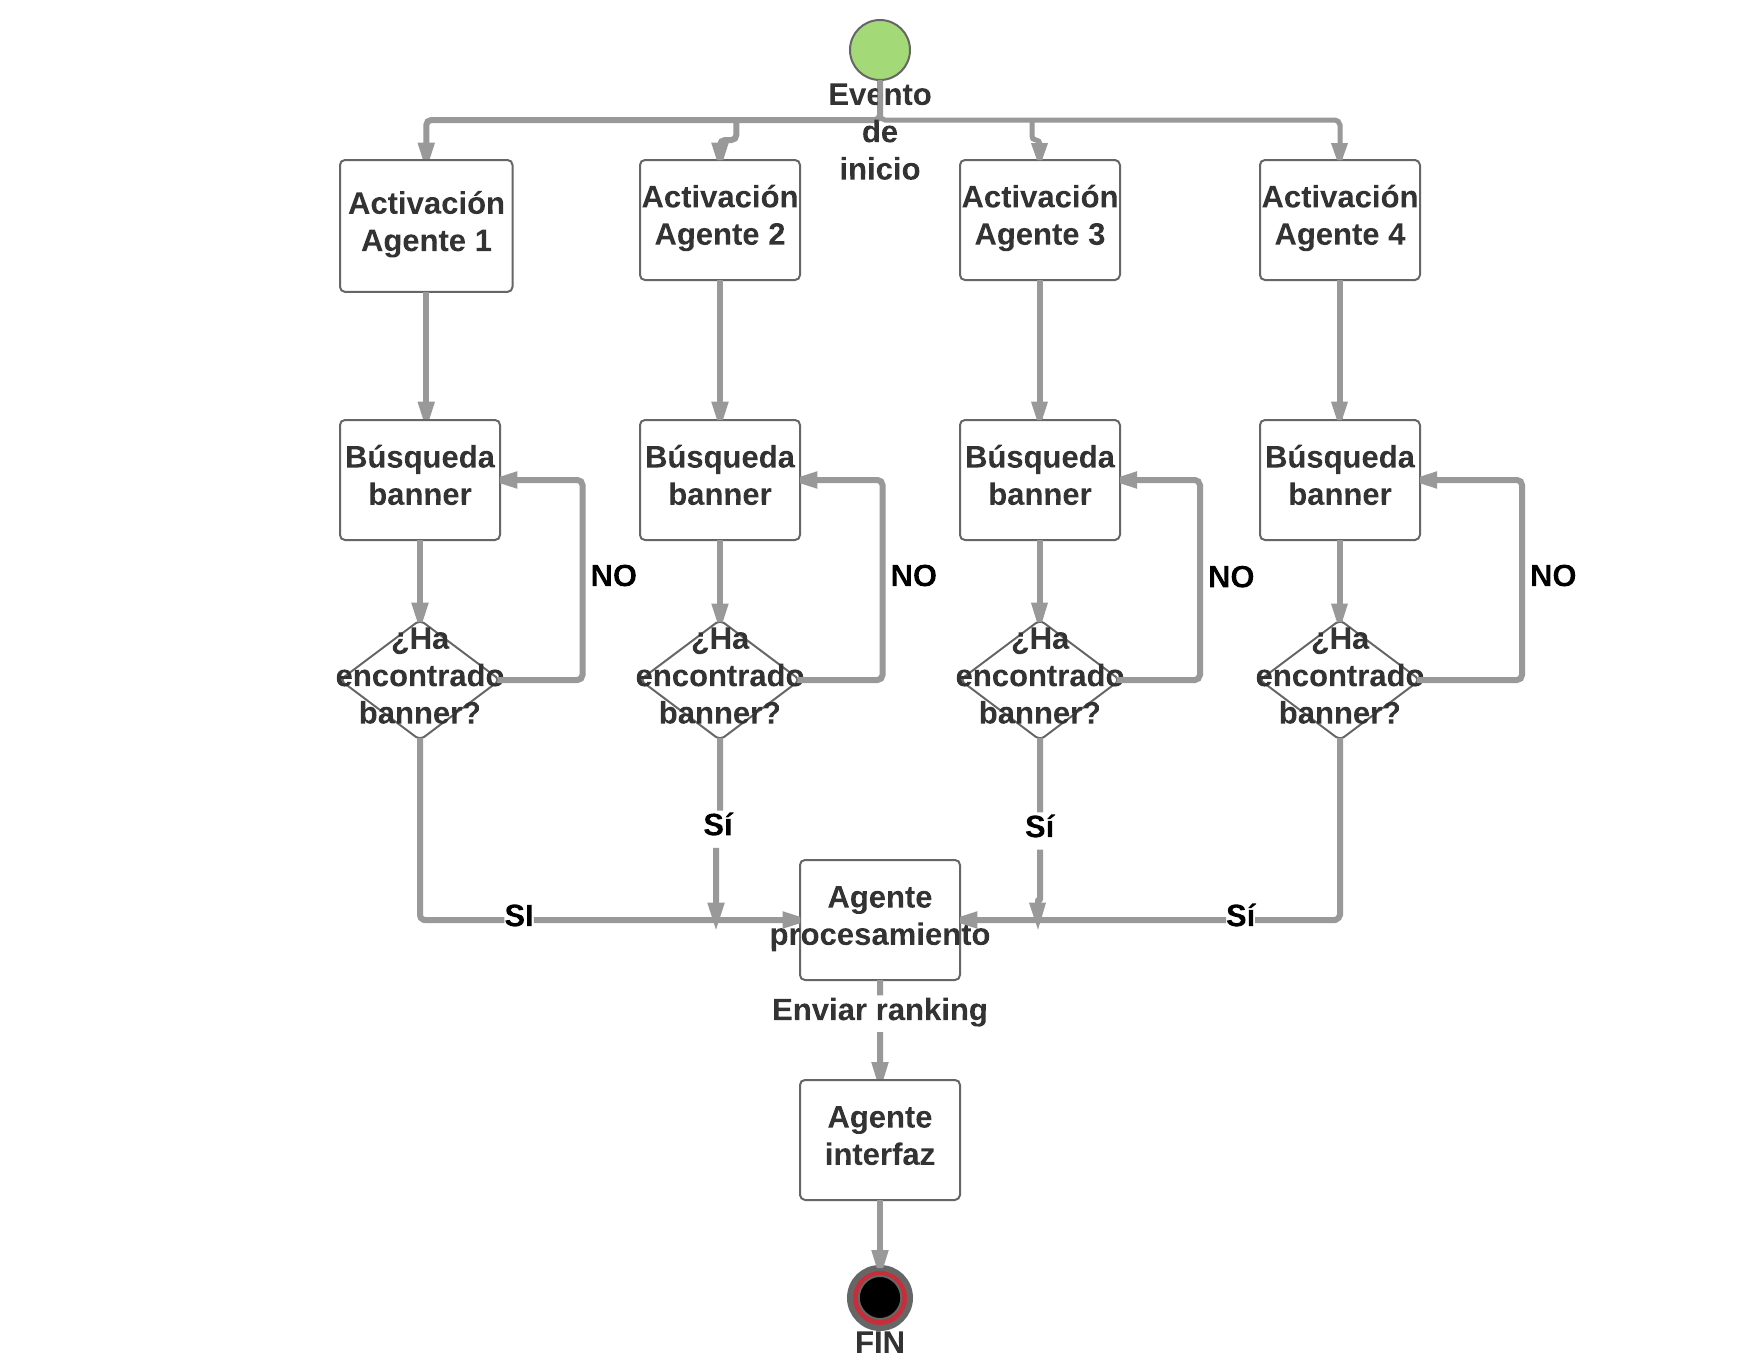
\includegraphics[width=1.0\textwidth]{flujo-sma}
    \caption{Diagrama de flujo del sistema multi-agente}
    \label{fig:flujo-sma}
\end{figure}

\clearpage

\section{MEDIOS QUE SE HAN UTILIZADO}
En el presente apartado se pretenden describir todos los medios que se utilizarán para llevar a cabo el proyecto
expuesto en este trabajo. Por un lado, se especificarán los medios hardware que se prevén necesarios para el desarrollo
del sistema. Por otro lado, se detallarán los medios software (lenguaje, entorno de desarrollo, herramientas de gestion y 
planificación, etc.) que se requieren para la construcción del presente proyecto.

\subsection{MEDIOS HARDWARE}
Para el desarrollo del sistema se ha requerido de dos equipos con sistemas \textit{Windows} y \textit{Linux}, dado
que los integrantes del grupo cuentan con ambos sistemas respectivamente. En cuanto a las especificaciones, ambos equipos
cuentan con unas caracterísitcas habituales por lo general, ya que no es necesario de un computador potente para el despliegue y desarrollo del
proyecto.

\subsection{MEDIOS SOFTWARE}

\begin{itemize}
 \item \textbf{Lenguaje}: para el desarrollo del sistema se ha utilizado el lenguaje Java, ya que la plataforma para el desarrollo 
 de agentes que se utilizará para la construcción del presente proyecto está implementada con el mismo.
 \item \textbf{Edición de código}: para la edición de código se ha utilizado el entorno \textit{Eclipse}, el cual facilita la escritura 
 del código debido al resaltado sintáctico que incorpora para el lenguaje Java.
 \item \textbf{Entorno de desarrollo}: el entorno a utilizar ha sido \textit{Eclipse}, debido a la facilidad mediante \textbf{JARs} de 
 integrar la plataforma para el desarrollo de agentes \textbf{JADE}, además del potente depurador que incorpora para ayudar a 
 corregir fallos en el código.
 \item \textbf{Orgnización}: se ha utilizado \textit{Git} como sistema de control de versiones y \textit{GitHub} como sistema web
 para la gestión de código. La elección de ambos sistemas se debe a la experiencia adquirida a lo largo de los últimos años de grado
 para el desarrollo de prácticas en diferentes asignaturas.
 \item \textbf{Documentación}: la documentación a desarrollar se ha hecho mediante el sistema de elaboración de textos \LaTeX.
\end{itemize}

\newpage

%%%%%%%%%%%%%%%%%%%%% ANEXOS %%%%%%%%%%%%%%%%%%%%%%%%%%%%%%%%%
\appendix
\section{CODIGO}

En el siguiente anexo se plasma el código que se ha desarrollado para la implementación del sistema multi-agente. Además,
se pretende explicar alguna de las partes que se consideran importantes para mejorar la comprensión del código y justificar
el porqué de su uso.

\subsection{EJEMPLO}

Este ejemplo simula el comportamiento que tendría un agente de recuperación de links en una página cualquiera.

\begin{lstlisting}[caption=Ejemplo de código de recuperación de links de una URL,style=java]

/**
 * Example program to list links from URL. 
 */
package sample;

import org.jsoup.Jsoup;
import org.jsoup.nodes.Document;
import org.jsoup.nodes.Element;
import org.jsoup.select.Elements;

import java.io.IOException;

/**
 * @author Alberto Aranda Garcia y Cristian Gomez Portes
 */
public class ListLinks {
    public static void main(String[] args) throws IOException {
        String url = "http://www.marca.com/"; // Test URL
        print("Fetching %s...", url);

        Document doc = Jsoup.connect(url).get();
        Elements links = doc.select("a[href]");
        Elements media = doc.select("[src]");

        print("\nMedia: (%d)", media.size());
        for (Element src : media) {
            if (src.tagName().equals("img"))
                print(" * %s: <%s> %sx%s (%s)",
                        src.tagName(), src.attr("abs:src"), src.attr("width"), src.attr("height"),
                        trim(src.attr("alt"), 20));
            else
                print(" * %s: <%s>", src.tagName(), src.attr("abs:src"));
        }

        print("\nLinks: (%d)", links.size());
        for (Element link : links) {
            print(" * a: <%s>  (%s)", link.attr("abs:href"), trim(link.text(), 35));
        }
    }

    private static void print(String msg, Object... args) {
        System.out.println(String.format(msg, args));
    }

    private static String trim(String s, int width) {
        if (s.length() > width)
            return s.substring(0, width-1) + ".";
        else
            return s;
    }
}

\end{lstlisting}

En el siguiente enlace se muestra el contenido del archivo ``blacklist'': \url{https://github.com/aarandag/ClassifiAds/blob/master/blacklist.txt}.

\clearpage

\bibliographystyle{alpha}
\singlespacing
\bibliography{ejemplo}

\end{document}

% Local Variables:
% coding: utf-8
% mode: flyspell
% ispell-local-dictionary: "castellano8"
% mode: latex
% End:
